\documentclass[11pt]{article}
\usepackage[margin=2cm]{geometry}
\usepackage{setspace}
\onehalfspacing
\usepackage{lineno}
\usepackage{graphicx}
\usepackage{float}

\title{%
 Project Proposal\\
 \LARGE Comparing the anadromous Atlantic salmon in Iceland and UK to research the impacts of temperature on Atlantic salmon}
\author{Yuxin Qin }
\date{December 2018}
\begin{document}
\maketitle
\begin{center}
    \Large Supervisor\\
    Guy Woodward\\
    Imperial College London\\
    guy.woodward@imperial.ac.uk
    \bigbreak
    \Large Co-supervisor\\
    James Rosindell\\
    Imperial College London\\
    j.rosindell@imperial.ac.uk
    \bigbreak
    \Large External supervisor\\
    Stephen Gregory\\
    GWCT
\end{center}

\newpage
\begin{linenumbers}
\section{Key words}
Bayesian Life-cycle Model; Population Ecology; Salmon; North Atlantic
\section{Introduction}
Atlantic salmon (\textit{Salmo salar}) are found to have two forms of life cycle in North Atlantic, the non-anadromous form and anadromous form \cite{verspoor2007atlantic}. The non-anadromous Atlantic salmon spend their entire life in a landlocked location, while the anadromous ones have more complicated life cycle. The anadromous Atlantic salmon are first born as eggs in freshwater, where they spend 2-4 years to slowly grow into smolts \cite{verspoor2007atlantic}. Then they go into the marine and live most of their time there except spawning. The first time of anadromous Atlantic salmon returning to spawn in rivers can range from 3 to 14 years after entering the sea \cite{chaput2012overview}. According to studies, both the smolt age and the sex mature age of anardromous Atlantic salmon is significantly dependent on temperature \cite{metcalfe1990determinants, scarnecchia1983age}. Regarding the steeply declination of native Atlantic salmon in North Atlantic since 1989 and the continuously ascending of global average marine temperature since 1950, temperature becomes a potential crucial factor that affects Atlantic salmon population and size \cite{parrish1998aren, brohan2006uncertainty}. Both located in North Atlantic, UK and Iceland has obvious different temperature during all season. Thus, the anadromous Atlantic salmon in Iceland and UK can be excellent examples to represent the cold area and warm area in North Atlantic, which helps study the impacts of temperature on anadromous Atlantic salmon. The population model of salmon in Iceland has already been completed by Hannah Levis. At the moment, the population model of salmon in UK is required to be constructed to compare with the ones in Iceland. 

\section{Methods}
The project is mainly conducted by computational methods. We intend to use Bayesian life-cycle model to construct the stage-structured population model of anadromous Atlantic salmon in UK. Bayesian life-cycle model is able to link different life stages of salmon and estimate stage-specific population of salmon under the effects of intrinsic and extrinsic factors \cite{ohlberger2018bayesian}. 

\section{Objectives}
The project is expected to construct the stage-structured population model of anadromous Atlantic salmon in UK. This model can improve stock assessment and calculation of conservation limits(CLs) and Quotas(QU), which provides both guidance on the conservation and fisheries. Further more, the project aims at comparing the anadromous Atlantic salmon between Iceland and UK to research the impacts of temperature on anadromous Atlantic salmon. 

\section{Project feasibility}
The project is part of the SAlmonoid MAnagement Round the CHannel(SAMARCH). SAMARCH is a €7.8m five-year project (2017-2022) part funded by the France England Interreg Channel programme. 
The timeline of tasks is listed Figure.1.
\begin{figure}[H]
   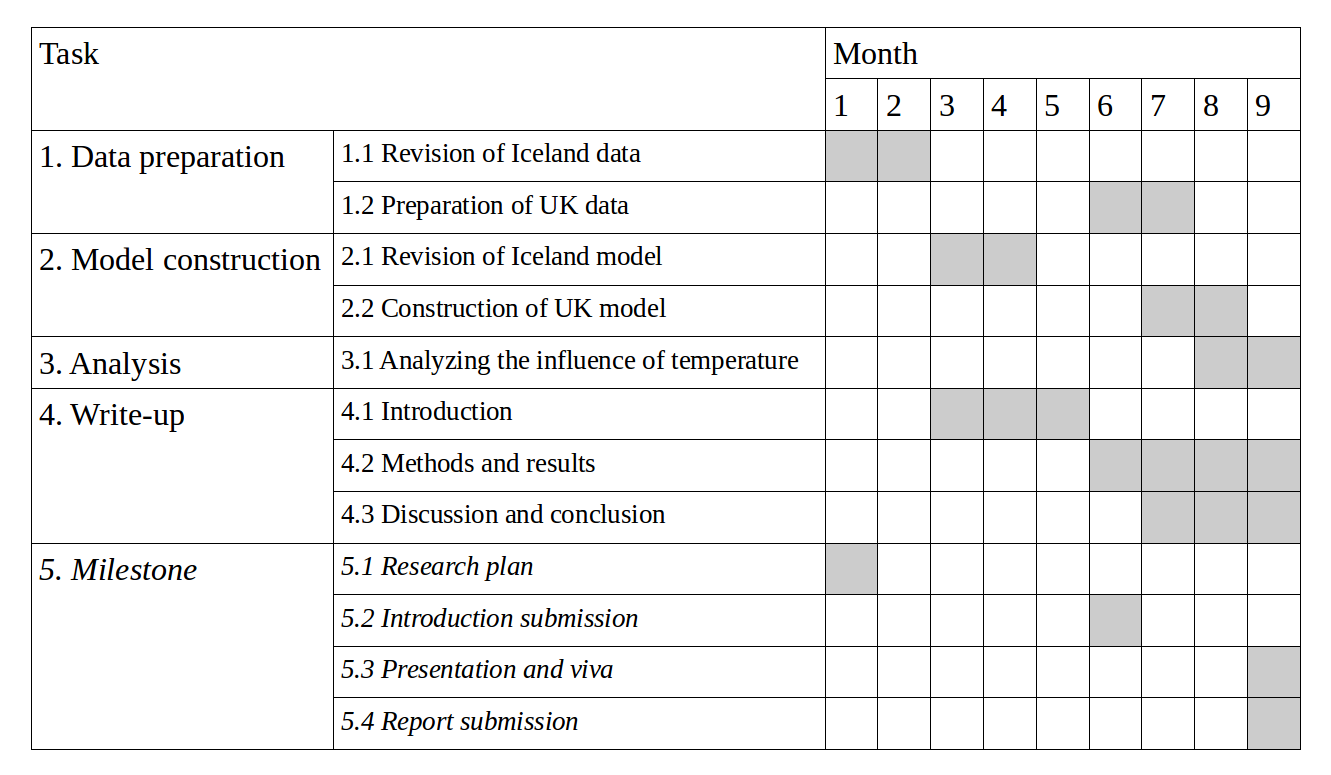
\includegraphics[width=\textwidth]{gantt_chart.png}
   \caption{Gantt chart of the project}
\end{figure}

\section{Budget}
The budget required is listed in table 1.
\begin{table}[H]
\centering
\begin{tabular}{ |c | c |}
 \hline
 &  Fee (\pounds)    \\
 \hline
 Transportation & 200     \\
 \hline
 Accommodation & 300     \\
 \hline
 Total & 500  \\
 \hline
\end{tabular}
\caption{Budget required for the project}
\end{table}

\newpage
\bibliographystyle{apalike}
\bibliography{bib.bib}

\end{linenumbers}


\newpage
\LARGE
I have seen and approved the proposal and the budget.
\bigbreak
\bigbreak
\bigbreak
\bigbreak
\large
Signature:
\bigbreak
\bigbreak
Date:
\end{document}